\begin{figure}[ht]
\centering
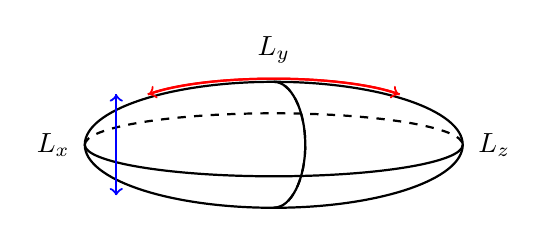
\begin{tikzpicture}[scale=0.8]
  % Draw the torus
  \draw[thick] (0,0) ellipse (3 and 1);
  \draw[thick] (0,-1) arc (-90:90:0.5 and 1);
  \draw[thick,dashed] (0,-1) arc (270:450:0.5 and 1);
  \draw[thick] (-3,0) arc (180:360:3 and 0.5);
  \draw[thick,dashed] (-3,0) arc (180:0:3 and 0.5);
  
  % Draw the identification arrows
  \draw[->,thick,blue] (-2.5,0.8) -- (-2.5,-0.8);
  \draw[->,thick,blue] (-2.5,-0.8) -- (-2.5,0.8);
  \draw[->,thick,red] (2,0.8) arc (30:150:2.3 and 0.5);
  \draw[->,thick,red] (-2,0.8) arc (150:30:2.3 and 0.5);
  
  % Labels
  \node at (-3.5,0) {$L_x$};
  \node at (0,1.5) {$L_y$};
  \node at (3.5,0) {$L_z$};
\end{tikzpicture}
\caption{Schematic representation of the Flat Loop Universe topology. The 3-torus structure is shown with identification of opposite faces (colored arrows), creating a finite but unbounded space with Euclidean local geometry.}
\label{fig:torus}
\end{figure}